\section{Results: do the classes separate?}
\label{sec:classes}

\subsection{The label check}

The original configurations sat at chance on motor imagery, and the labels are not the reason. Imagining the right hand lowers mu power over the left hemisphere, and the left hand lowers it over the right \cite{pfurtscheller1999}. In the raw spectra (Fig.~\ref{fig:spectra}), right minus left hand on EEG MMI is \N{sp:eeg_mmi:C3..:12:mean} dB at C3 [\N{sp:eeg_mmi:C3..:12:lo}, \N{sp:eeg_mmi:C3..:12:hi}] and \N{sp:eeg_mmi:C4..:12:mean} dB at C4 [\N{sp:eeg_mmi:C4..:12:lo}, \N{sp:eeg_mmi:C4..:12:hi}] at 12 Hz, and in the average of C3, Cz, and C4, it nearly cancels (\N{sp:eeg_mmi:average:12:mean} dB [\N{sp:eeg_mmi:average:12:lo}, \N{sp:eeg_mmi:average:12:hi}]). On BCI IV 2a, the direction is the same with wide intervals, \N{sp:bci_civ_2a:EEG-C3:12:mean} dB at C3 [\N{sp:bci_civ_2a:EEG-C3:12:lo}, \N{sp:bci_civ_2a:EEG-C3:12:hi}] and \N{sp:bci_civ_2a:EEG-C4:12:mean} dB at C4 [\N{sp:bci_civ_2a:EEG-C4:12:lo}, \N{sp:bci_civ_2a:EEG-C4:12:hi}] (9 subjects, so ``same direction, wide intervals''). The original pipeline averaged the channels and z-scored each window, which removes most of this signal. The intervals are pointwise at 45 frequencies, and the quoted bins are the observed mu-band peaks.

\begin{figure}[t]
\centering
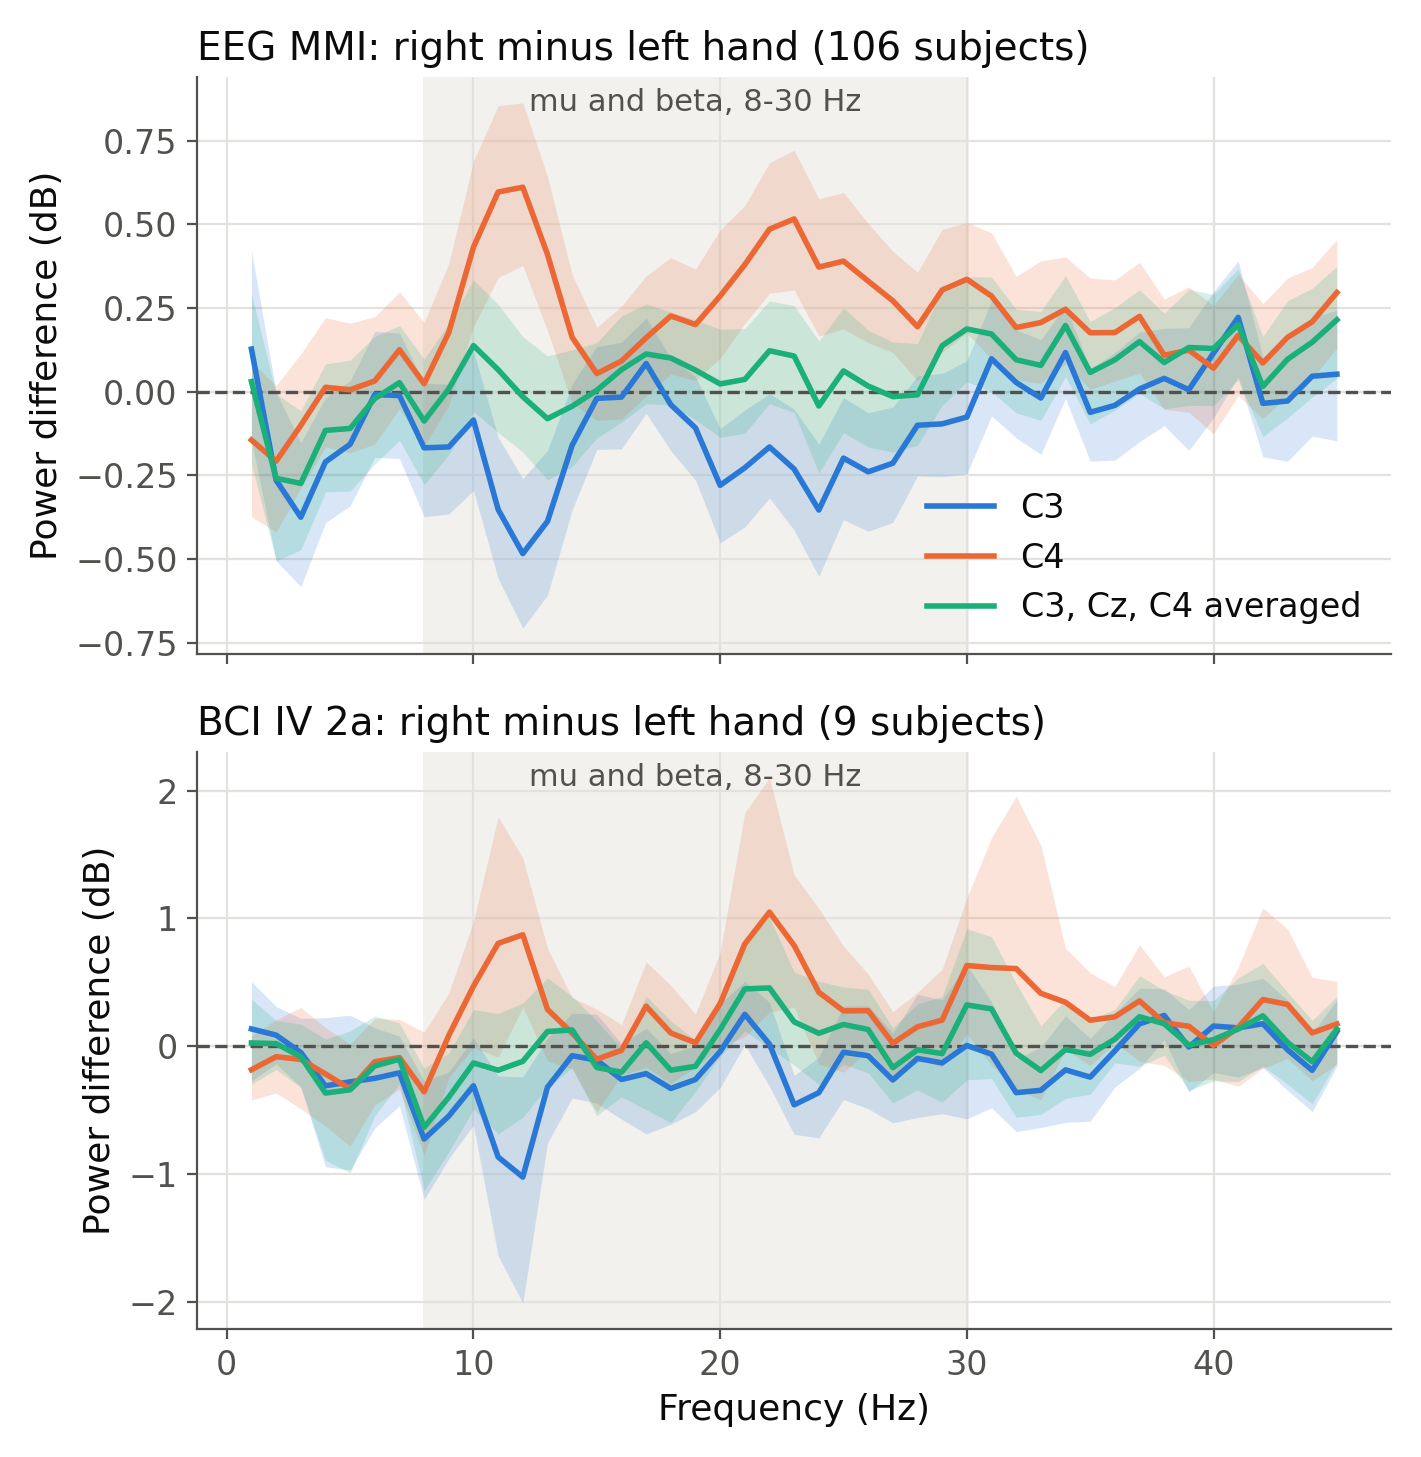
\includegraphics[width=\columnwidth]{../results/study/figures/fig4_spectra.png}
\caption{Right-minus-left-hand spectra at C3 and C4 and for the average of C3, Cz, and C4, for EEG MMI and BCI IV 2a, with 95\% bands; the 8--30 Hz range is shaded.}
\label{fig:spectra}
\end{figure}

\subsection{Held-out subjects}

With channels kept separate, band power with LDA classifies held-out subjects above chance (Table~\ref{tab:lda} and Fig.~\ref{fig:heldout}). With each subject's features standardized over its own unlabeled windows, balanced accuracy is \N{sm:eeg_mmi:F1_ch:lda:heldout:subject} [\N{sm:eeg_mmi:F1_ch:lda:heldout:subject:lo}, \N{sm:eeg_mmi:F1_ch:lda:heldout:subject:hi}] on EEG MMI, \N{sm:bci_civ_2a:F1_ch:lda:heldout:subject} [\N{sm:bci_civ_2a:F1_ch:lda:heldout:subject:lo}, \N{sm:bci_civ_2a:F1_ch:lda:heldout:subject:hi}] on BCI IV 2a, and \N{sm:eeg_ma:F1_ch:lda:heldout:subject} [\N{sm:eeg_ma:F1_ch:lda:heldout:subject:lo}, \N{sm:eeg_ma:F1_ch:lda:heldout:subject:hi}] on EEGMAT. Without standardizing, the values are \N{sm:eeg_mmi:F1_ch:lda:heldout:none}, \N{sm:bci_civ_2a:F1_ch:lda:heldout:none}, and \N{sm:eeg_ma:F1_ch:lda:heldout:none}, still above chance. With per-subject permutation tests at \N{c:perm_subject_shuffles} shuffles, \N{sm:eeg_mmi:F1_ch:lda:heldout:subject:bh} of 106, \N{sm:bci_civ_2a:F1_ch:lda:heldout:subject:bh} of 9, and \N{sm:eeg_ma:F1_ch:lda:heldout:subject:bh} of 36 subjects are above chance after correction with standardizing, and \N{sm:eeg_mmi:F1_ch:lda:heldout:none:bh}, \N{sm:bci_civ_2a:F1_ch:lda:heldout:none:bh}, and \N{sm:eeg_ma:F1_ch:lda:heldout:none:bh} without. These tests shuffle window labels freely, which assumes exchangeable windows; on EEGMAT, where each class is one recording, they show at most that a subject's two recordings differ, not that the task does.

\begin{table*}[t]
\caption{LDA: mean per-subject balanced accuracy with a 95\% interval over subjects (number of subjects in parentheses). Chance is 0.50 for EEG MMI and EEGMAT and 0.25 for BCI IV 2a. ``Standardized'' means within each held-out subject over all its unlabeled windows.}
\label{tab:lda}
\centering
\scriptsize
\setlength{\tabcolsep}{4pt}
\begin{tabular}{@{}llccc@{}}
\toprule
Data set & Features & Within subject & Held out, as is & Held out, standardized \\
\midrule
EEG MMI (106) & Band power, averaged & 0.527 [0.511, 0.543] & 0.509 [0.498, 0.519] & 0.509 [0.493, 0.524] \\
 & Band power, per channel & 0.549 [0.525, 0.572] & 0.569 [0.550, 0.588] & 0.595 [0.573, 0.616] \\
 & IMF features, per channel & 0.493 [0.475, 0.511] & 0.544 [0.528, 0.562] & 0.575 [0.557, 0.594] \\
 & Hilbert band power, per channel & 0.533 [0.513, 0.555] & 0.558 [0.543, 0.574] & 0.589 [0.570, 0.607] \\
\midrule
BCI IV 2a (9) & Band power, averaged & 0.291 [0.263, 0.325] & 0.255 [0.241, 0.272] & 0.283 [0.266, 0.299] \\
 & Band power, per channel & 0.432 [0.371, 0.508] & 0.315 [0.291, 0.343] & 0.372 [0.325, 0.424] \\
 & IMF features, per channel & 0.327 [0.274, 0.398] & 0.274 [0.260, 0.290] & 0.340 [0.303, 0.386] \\
 & Hilbert band power, per channel & 0.384 [0.335, 0.440] & 0.308 [0.292, 0.323] & 0.374 [0.330, 0.432] \\
\midrule
EEGMAT (36) & Band power, averaged & 0.747 [0.711, 0.783] & 0.530 [0.512, 0.551] & 0.577 [0.549, 0.606] \\
 & Band power, per channel & 0.946 [0.928, 0.962] & 0.593 [0.555, 0.639] & 0.692 [0.642, 0.743] \\
 & IMF features, per channel & 0.912 [0.881, 0.942] & 0.580 [0.544, 0.626] & 0.664 [0.617, 0.715] \\
 & Hilbert band power, per channel & 0.947 [0.929, 0.965] & 0.586 [0.544, 0.633] & 0.698 [0.650, 0.749] \\
\bottomrule
\end{tabular}

\end{table*}

\begin{figure}[t]
\centering
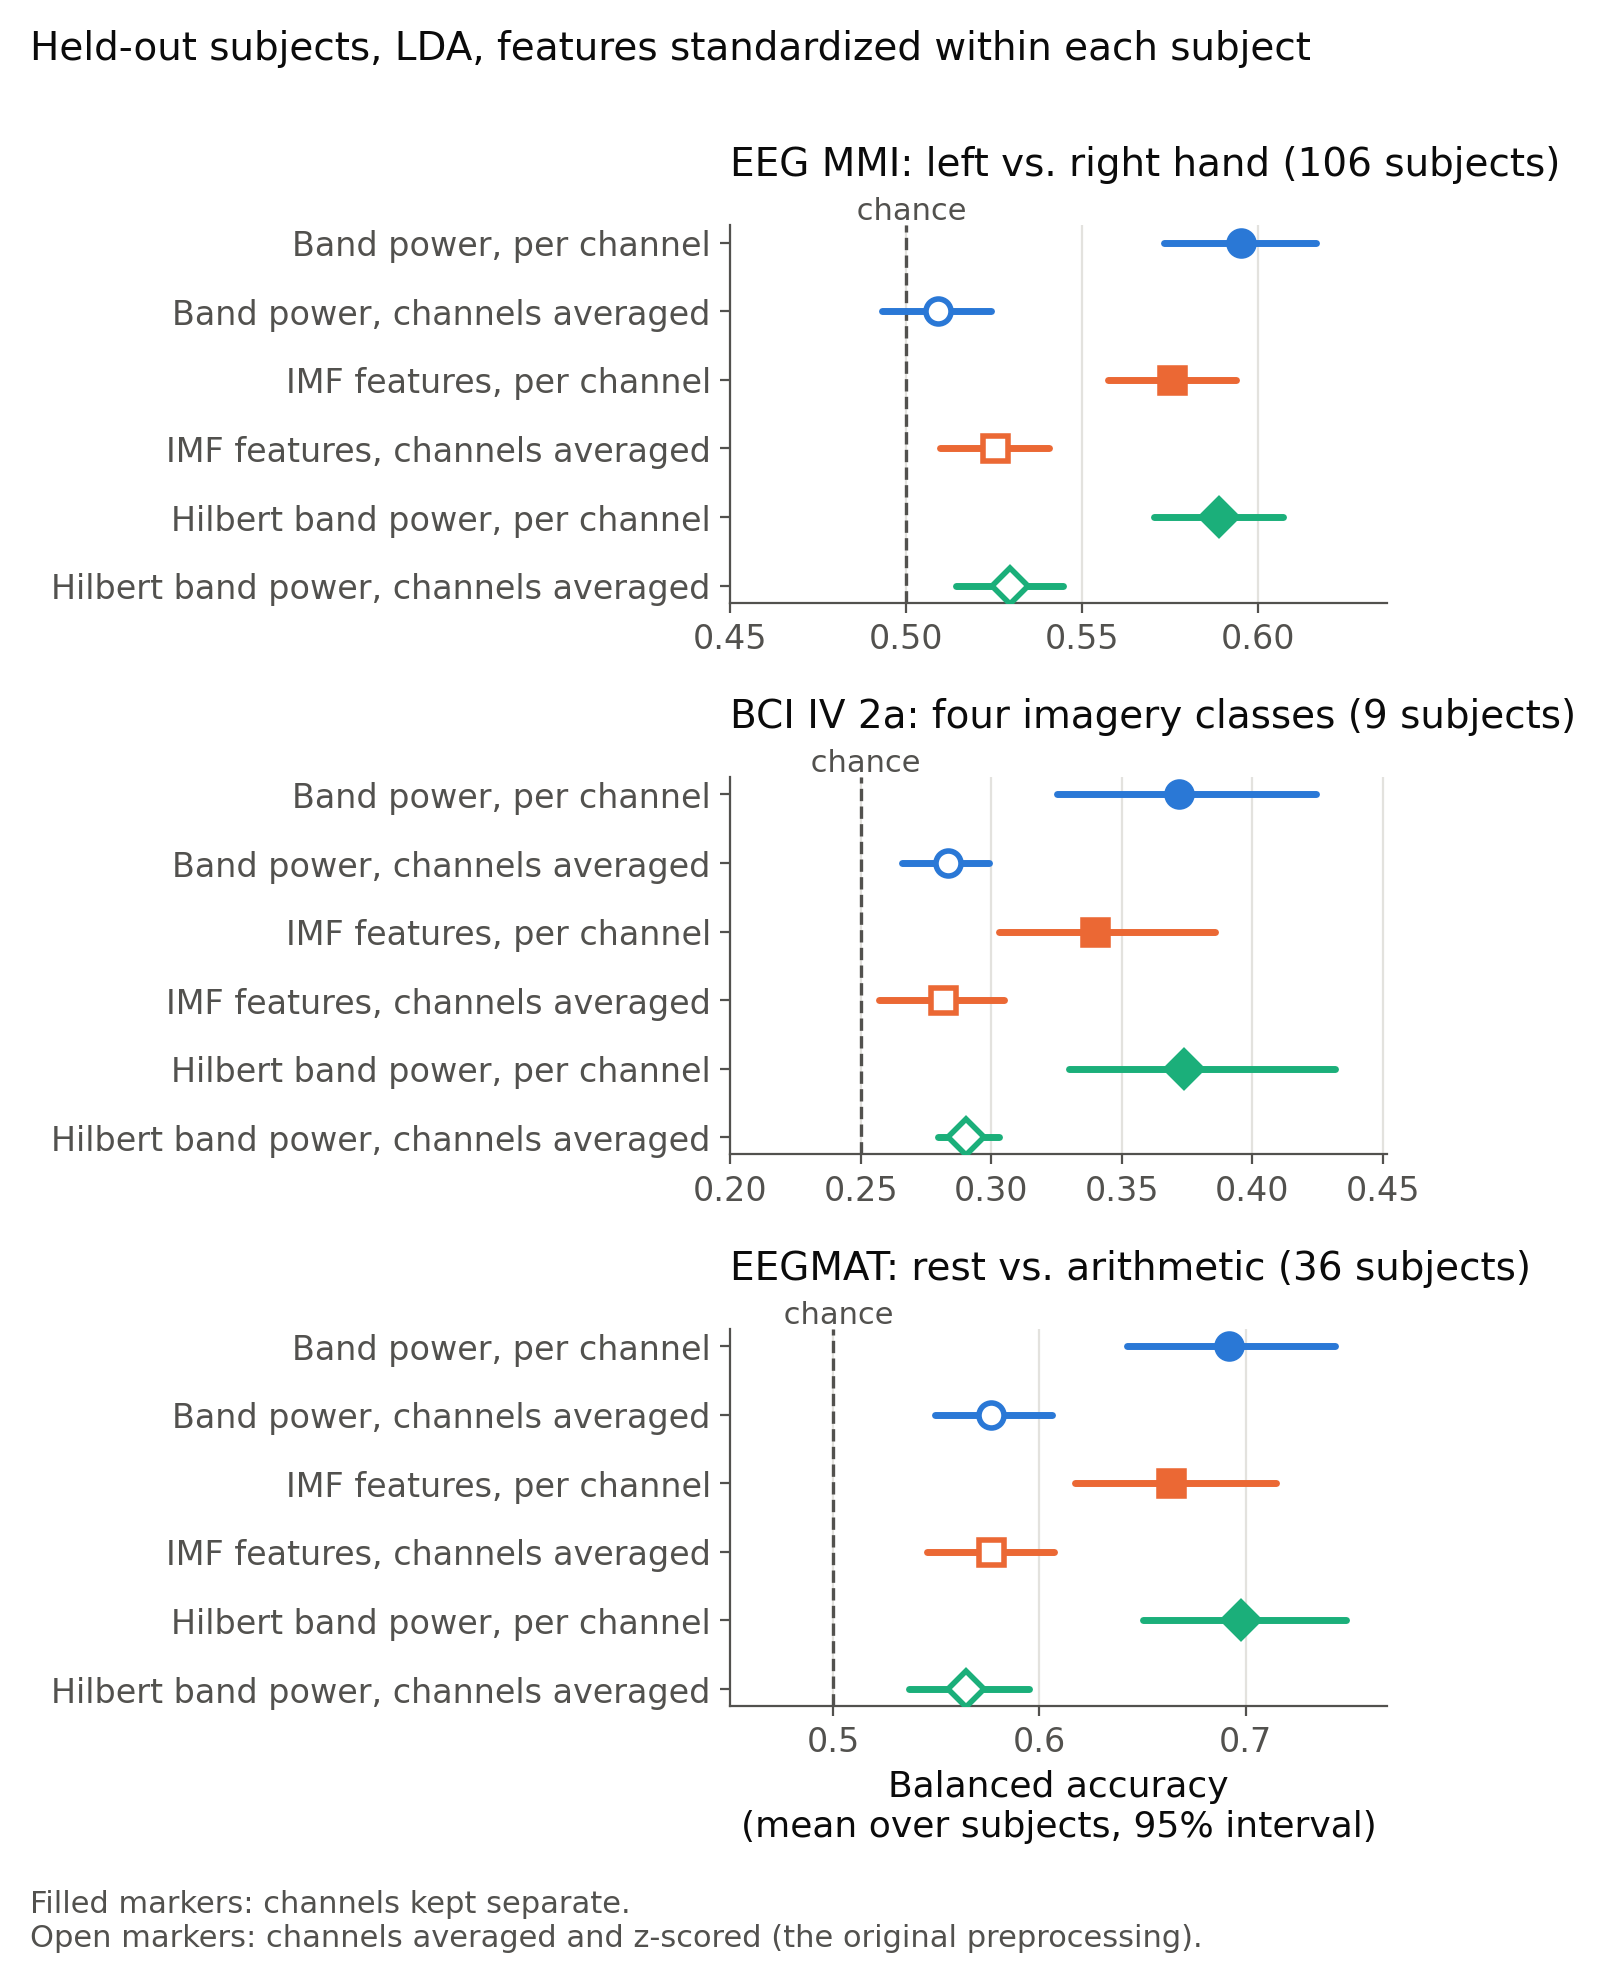
\includegraphics[width=\columnwidth]{../results/study/figures/fig1_heldout.png}
\caption{Held-out subjects, LDA, features standardized within each subject: balanced accuracy for six feature sets on each data set, with 95\% intervals and the chance line.}
\label{fig:heldout}
\end{figure}

\emph{Averaging the channels costs most of it.} On held-out subjects (LDA, standardized), per-channel features beat their averaged versions by \N{c:avgcost_min} to \N{c:avgcost_max} (\N{c:avgcost_none_min} to \N{c:avgcost_none_max} unstandardized). The averaged versions are also z-scored per window, as in the original pipeline, while the per-channel ones are only detrended, so this gap measures both changes together. The gain from keeping channels apart for band power is \N{pt:eeg_mmi:heldout:subject:lda:F1_ch:F1_avg} on EEG MMI (Holm $p$ \N{pt:eeg_mmi:heldout:subject:lda:F1_ch:F1_avg:ph}) and \N{pt:eeg_ma:heldout:subject:lda:F1_ch:F1_avg} on EEGMAT (\N{pt:eeg_ma:heldout:subject:lda:F1_ch:F1_avg:ph}); unstandardized, it is \N{pt:eeg_mmi:heldout:none:lda:F1_ch:F1_avg} (\N{pt:eeg_mmi:heldout:none:lda:F1_ch:F1_avg:ph}) and \N{pt:eeg_ma:heldout:none:lda:F1_ch:F1_avg} (\N{pt:eeg_ma:heldout:none:lda:F1_ch:F1_avg:ph}). On BCI IV 2a, \N{ps:bci_civ_2a:F1} of the 9 subjects improve for band power, \N{ps:bci_civ_2a:F3} for Hilbert band power, and \N{ps:bci_civ_2a:F2} for the IMF features (\N{ps:bci_civ_2a:F1:none}, \N{ps:bci_civ_2a:F3:none}, and \N{ps:bci_civ_2a:F2:none} unstandardized), and no 9-subject comparison can pass Holm.

\subsection{Where the EEGMAT result comes from}

Within subjects, band power per channel on EEGMAT scores \N{sm:eeg_ma:F1_ch:lda:within:none} [\N{sm:eeg_ma:F1_ch:lda:within:none:lo}, \N{sm:eeg_ma:F1_ch:lda:within:none:hi}], but rest is recorded first, in its own file, so within a subject the classifier can tell the two recordings apart. Holding subjects out removes subject identity and not that. Table~\ref{tab:eegmat} shows where the held-out accuracy comes from. Without the frontal-polar channels Fp1 and Fp2, it falls to \N{es:without Fp1 and Fp2:subject} (\N{es:without Fp1 and Fp2:none} unstandardized), a loss of \N{mag:es:without Fp1 and Fp2:subject:diff} [\N{mag:es:without Fp1 and Fp2:subject:diffhi}, \N{mag:es:without Fp1 and Fp2:subject:difflo}] (\N{mag:es:without Fp1 and Fp2:none:diff} unstandardized). The two channels alone give \N{es:Fp1 and Fp2 only:subject} (\N{es:Fp1 and Fp2 only:none} unstandardized), and the alpha band alone, where the cortical effect of mental arithmetic is expected, gives \N{es:alpha band only:subject} (\N{es:alpha band only:none} unstandardized). The largest class differences at Fp1 and Fp2 are slow (1 to 6 Hz) and fast (25 to 45 Hz) power, the usual signature of eye movements and muscle activity, while alpha is lower at every channel, most at F3, F4, and Fz and in the channel average. The data set's documentation reports that eye, muscle, and cardiac artifacts were removed with independent component analysis \cite{eegmat}, so any such activity left would be residual. The held-out EEGMAT number may partly reflect recording order and non-cortical activity, and it does not by itself show a cortical effect of mental arithmetic.

\begin{table}[t]
\caption{EEGMAT, band power per channel, LDA, leave one subject out: mean per-subject balanced accuracy [95\% interval] for subsets of the channels and bands. No.: number of features; ``Standardized'': within each held-out subject. The first row is from the main summary, as in Table~\ref{tab:lda}; the other rows come from a separate run of the subsets, whose intervals use their own bootstrap draws.}
\label{tab:eegmat}
\centering
\scriptsize
\setlength{\tabcolsep}{2pt}
\begin{tabular}{@{}lccc@{}}
\toprule
Features & No. & Standardized & As is \\
\midrule
All channels and bands & 25 & 0.692 [0.642, 0.743] & 0.593 [0.555, 0.639] \\
Without Fp1, Fp2 & 15 & 0.553 [0.532, 0.576] & 0.520 [0.502, 0.540] \\
Fp1, Fp2 only & 10 & 0.665 [0.619, 0.713] & 0.571 [0.531, 0.612] \\
Alpha band only & 5 & 0.531 [0.513, 0.553] & 0.512 [0.498, 0.531] \\
Without 1--4, 30--45 Hz & 15 & 0.627 [0.586, 0.671] & 0.572 [0.534, 0.615] \\
\bottomrule
\end{tabular}

\end{table}

\subsection{The window split overstates accuracy}

On the original 70/30 split of windows, Euclidean KNN on EEGMAT with per-channel band power scores \N{ss:eeg_ma:F1_ch:knn_euclidean:mean} (seeds 0 to 9) against \N{sm:eeg_ma:F1_ch:knn_euclidean:heldout:none} on held-out subjects without standardizing (Fig.~\ref{fig:leak}): neighboring windows of one recording, and one recording per class. With LDA, the gap is smaller, \N{ss:eeg_ma:F1_ch:lda:mean} against \N{sm:eeg_ma:F1_ch:lda:heldout:none}. On BCI IV 2a, the split is also higher, KNN \N{ss:bci_civ_2a:F1_ch:knn_euclidean:mean} (range \N{ss:bci_civ_2a:F1_ch:knn_euclidean:min} to \N{ss:bci_civ_2a:F1_ch:knn_euclidean:max}) against \N{sm:bci_civ_2a:F1_ch:knn_euclidean:heldout:none} and LDA \N{ss:bci_civ_2a:F1_ch:lda:mean} against \N{sm:bci_civ_2a:F1_ch:lda:heldout:none}, because each subject's windows are on both sides of the split. On EEG MMI, the two agree (KNN \N{ss:eeg_mmi:F1_ch:knn_euclidean:mean} and \N{sm:eeg_mmi:F1_ch:knn_euclidean:heldout:none}; LDA \N{ss:eeg_mmi:F1_ch:lda:mean} and \N{sm:eeg_mmi:F1_ch:lda:heldout:none}).

\begin{figure}[t]
\centering
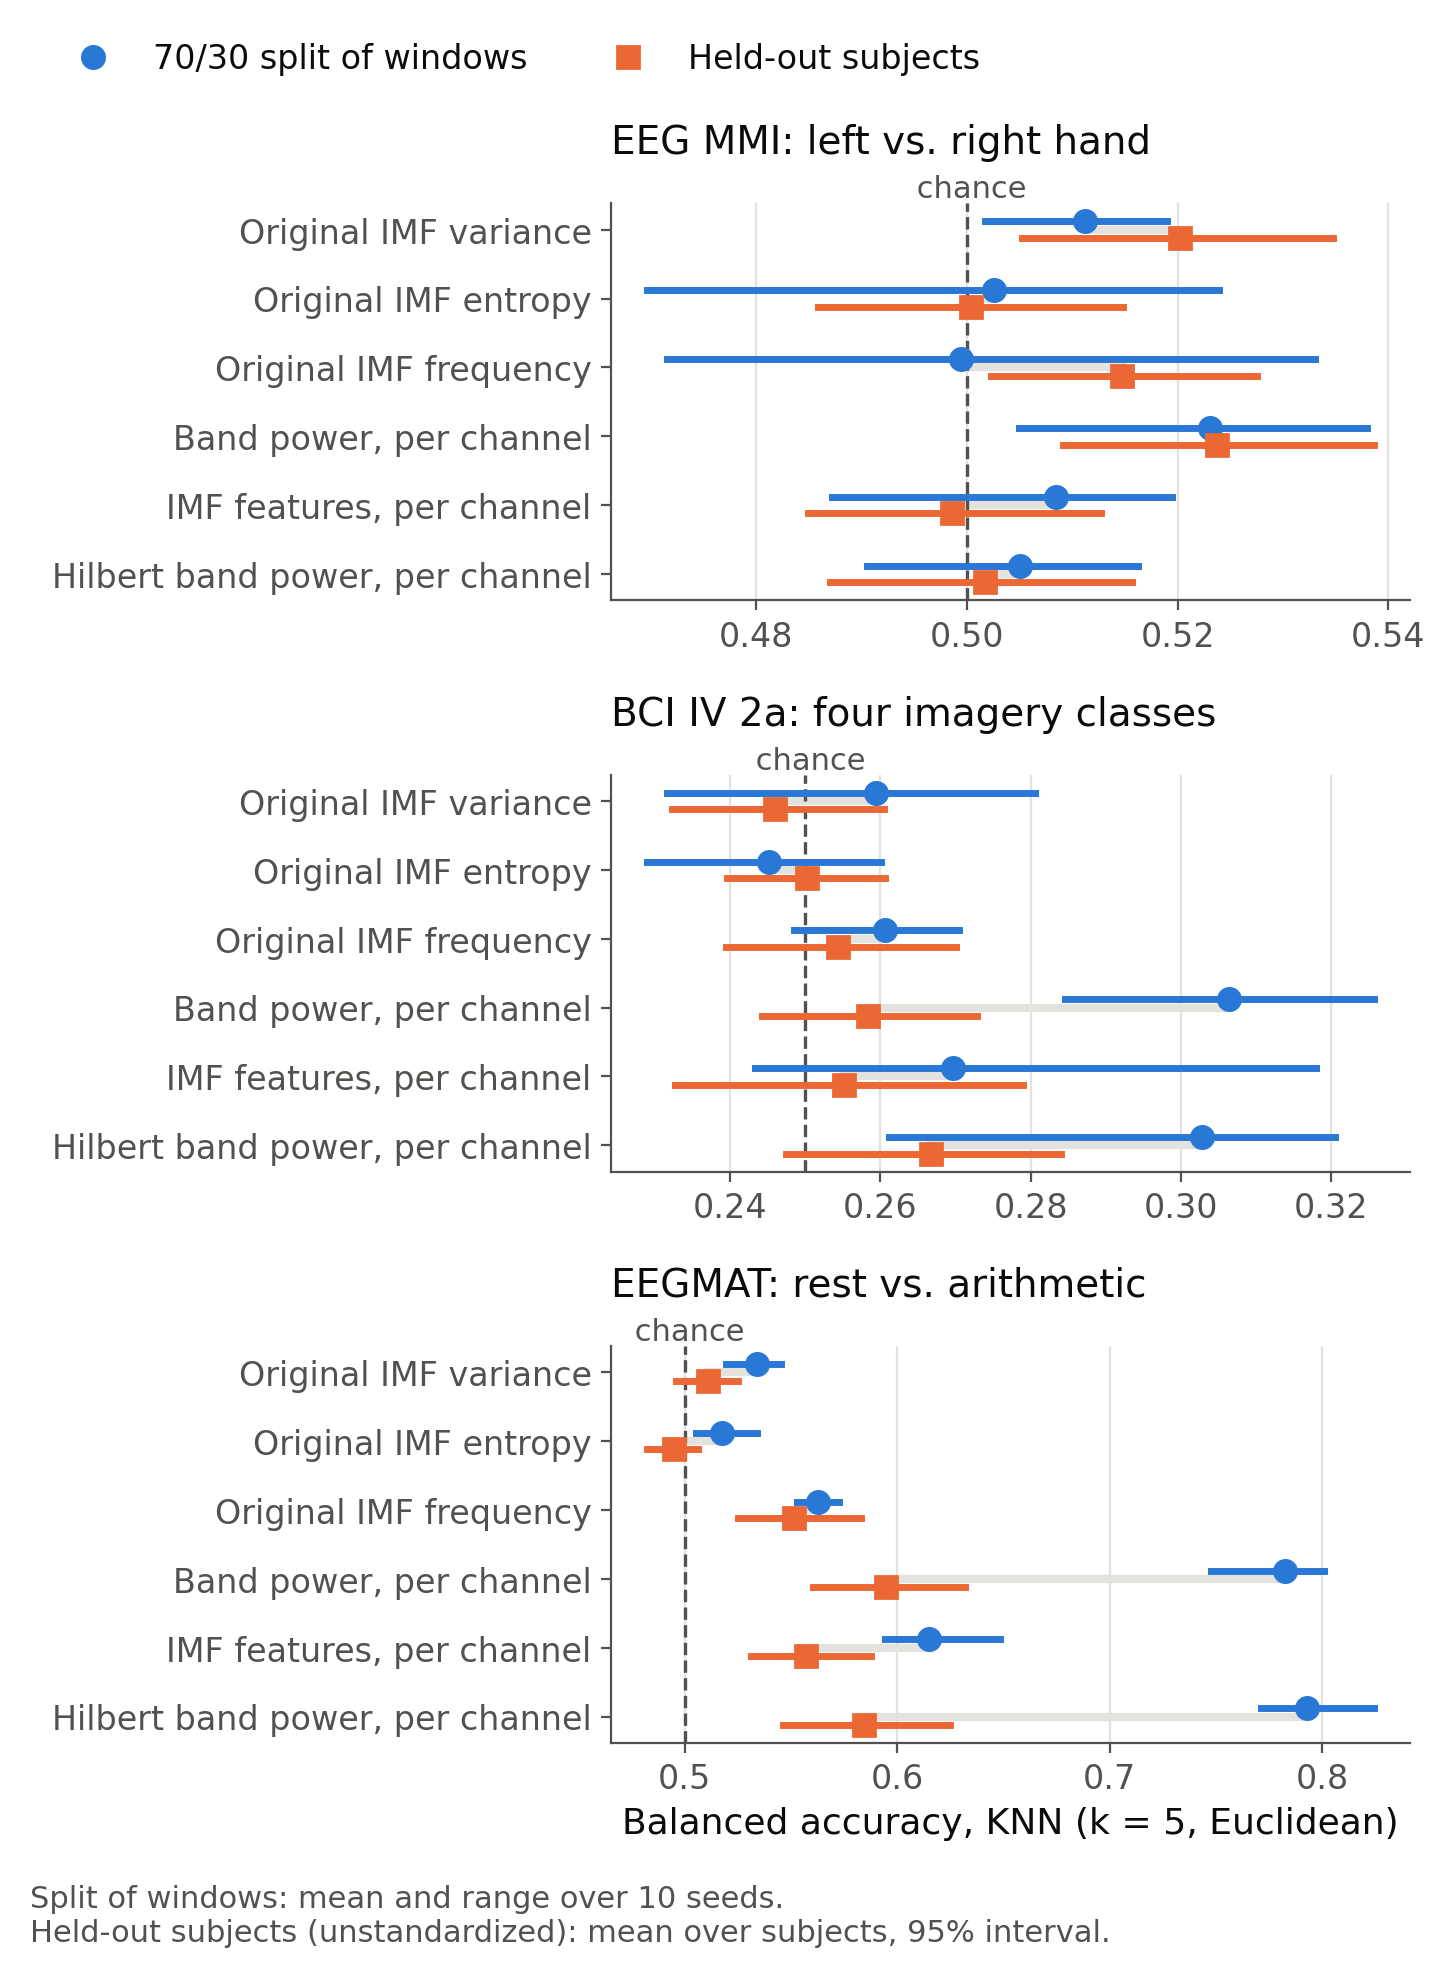
\includegraphics[width=\columnwidth]{../results/study/figures/fig5_leak.png}
\caption{Euclidean KNN on the original window split against held-out subjects, six feature sets per data set. The held-out points use the features as they are.}
\label{fig:leak}
\end{figure}

\emph{The original features stay at chance.} Over the nine F0 configurations and the three subject-based evaluations, EEG MMI scores \N{c:f0_range:eeg_mmi} and BCI IV 2a \N{c:f0_range:bci_civ_2a}. Of these \N{c:f0_n} intervals, \N{c:f0_excl} exclude chance, with means at most \N{c:f0_excl_max} from it, about as many as chance alone would give (\N{c:f0_expected} expected at the 5\% level).
